% Copyright (c)  2019  FSC.
% Permission is granted to copy, distribute and/or modify this document
% under the terms of the GNU Free Documentation License, Version 1.3
% or any later version published by the Free Software Foundation;
% with no Invariant Sections, no Front-Cover Texts, and no Back-Cover Texts.
% A copy of the license is included in the section entitled "GNU
% Free Documentation License".

\begin{figure}[H]
	\centering
	\caption{Diagramma macchine a stati del caso d'uso 'Registration'.}
	\label{fig:diagramma-macchine-stati:registration}
	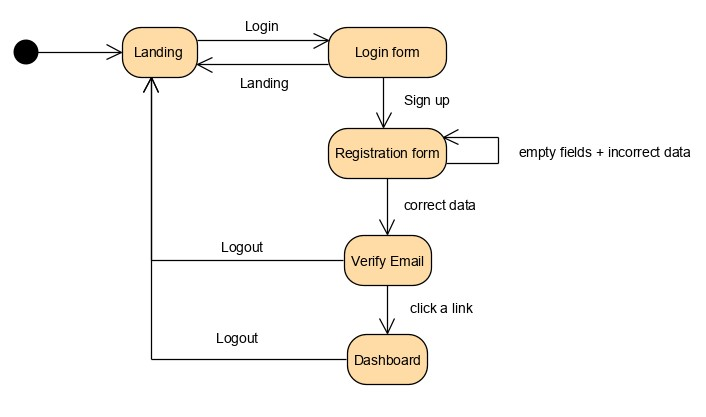
\includegraphics[width=\textwidth]{images/diagramma-macchine-stati/registration}
\end{figure}

\begin{figure}[H]
	\centering
	\caption{Diagramma macchine a stati del caso d'uso 'Login'.}
	\label{fig:diagramma-macchine-stati:login}
	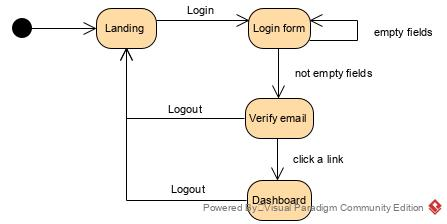
\includegraphics[width=\textwidth]{images/diagramma-macchine-stati/login}
\end{figure}
\begin{figure}[H]
	\centering

	\caption{Diagramma macchine a stati del caso d'uso 'Logout'.}
	\label{fig:diagramma-macchine-stati:logout}
	
\includegraphics[width=\textwidth]{images/diagramma-macchine-stati/logout}
\end{figure}

\begin{figure}[H]
	\centering
	\caption{Diagramma macchine a stati del caso d'uso 'Create project'.}
	\label{fig:diagramma-macchine-stati:create-project}
	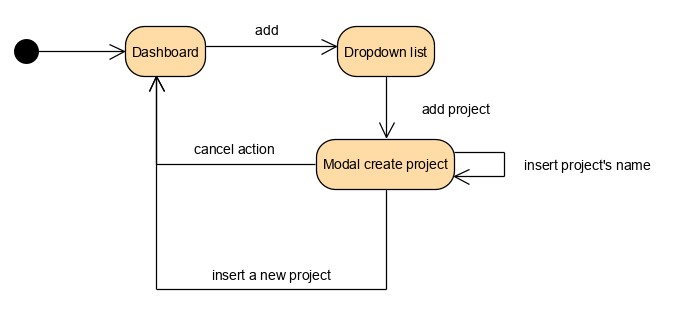
\includegraphics[width=\textwidth]{images/diagramma-macchine-stati/create-project}
\end{figure}

\begin{figure}[H]
	\centering
	\caption{Diagramma macchine a stati del caso d'uso 'View project'.}
	\label{fig:diagramma-macchine-stati:view-project}
	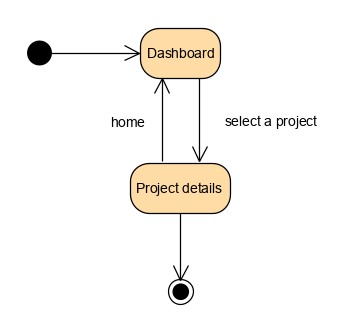
\includegraphics[width=\textwidth]{images/diagramma-macchine-stati/view-project}
\end{figure}


\begin{figure}[H]
	\centering
	\caption{Diagramma macchine a stati del caso d'uso 'Edit project'.}
	\label{fig:diagramma-macchine-stati:edit-project}
	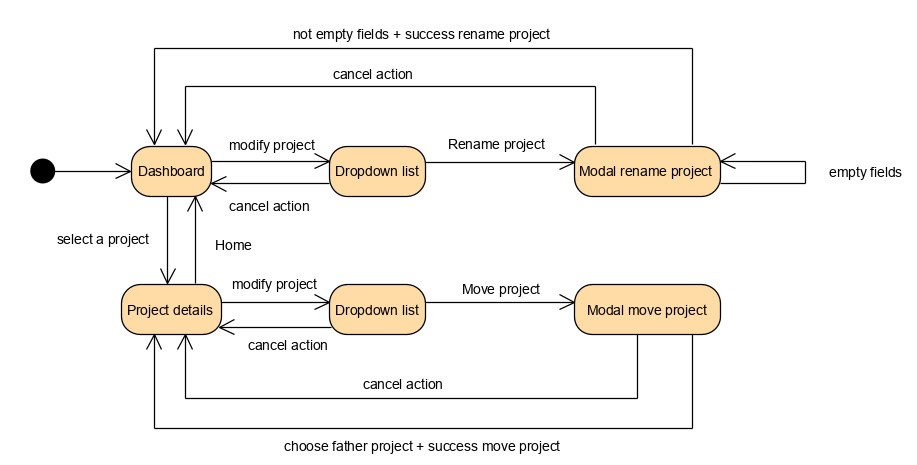
\includegraphics[width=\textwidth]{images/diagramma-macchine-stati/edit-project}
\end{figure}

\begin{figure}[H]
	\centering
	\caption{Diagramma macchine a stati del caso d'uso 'Remove project'.}
	\label{fig:diagramma-macchine-stati:remove-project}
	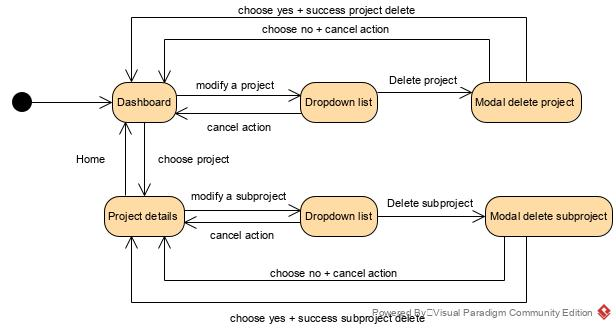
\includegraphics[width=\textwidth]{images/diagramma-macchine-stati/remove-project}
\end{figure}

\begin{figure}[H]
	\centering
	\caption{Diagramma macchine a stati del caso d'uso 'Upload video'.}
	\label{fig:diagramma-macchine-stati:upload-video}
	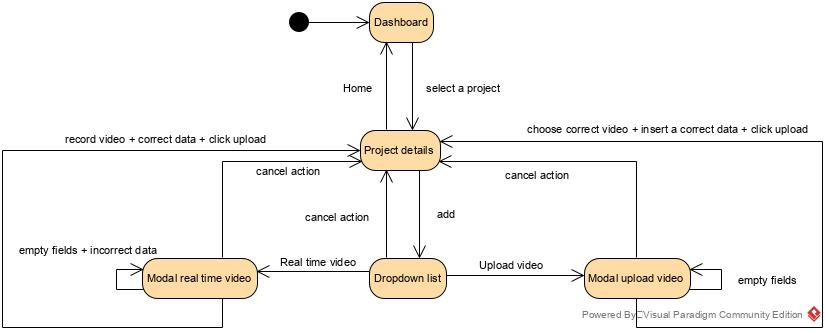
\includegraphics[width=\textwidth]{images/diagramma-macchine-stati/upload-video}
\end{figure}

\begin{figure}[H]
	\centering
	\caption{Diagramma macchine a stati del caso d'uso 'Edit video'.}
	\label{fig:diagramma-macchine-stati:edit-video}
	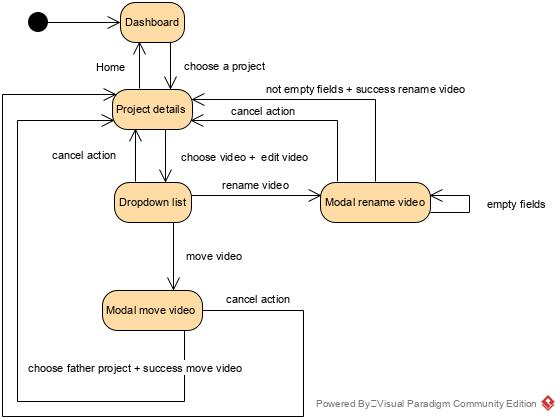
\includegraphics[width=\textwidth]{images/diagramma-macchine-stati/edit-video}
\end{figure}

\begin{figure}[H]
	\centering
	\caption{Diagramma macchine a stati del caso d'uso 'Remove video'.}
	\label{fig:diagramma-macchine-stati:remove-video}
	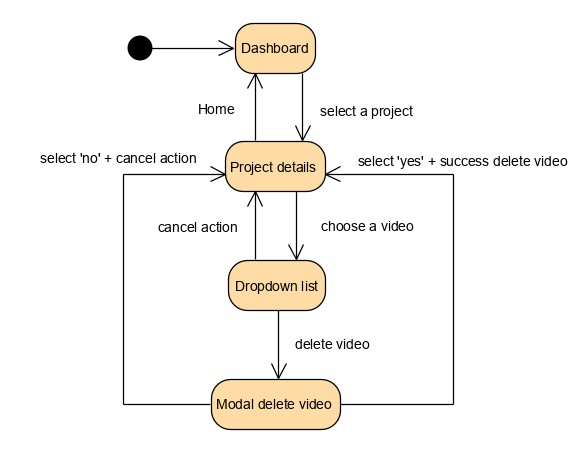
\includegraphics[width=\textwidth]{images/diagramma-macchine-stati/remove-video}
\end{figure}

\begin{figure}[H]
	\centering
	\caption{Diagramma macchine a stati del caso d'uso 'View video'.}
	\label{fig:diagramma-macchine-stati:view-video}
	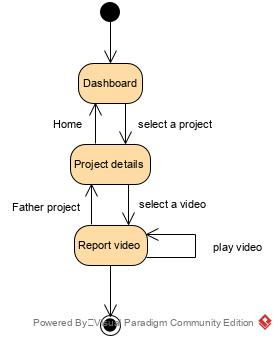
\includegraphics[width=\textwidth]{images/diagramma-macchine-stati/view-video}
\end{figure}

\begin{figure}[H]
	\centering
	\caption{Diagramma macchine a stati del caso d'uso 'Share project'.}
	\label{fig:diagramma-macchine-stati:share-project}
	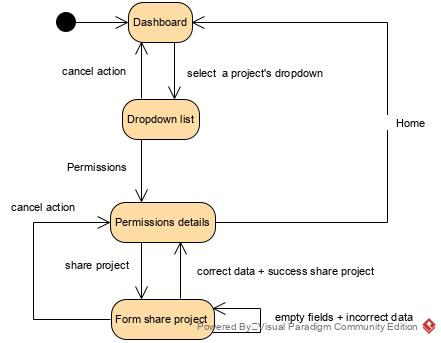
\includegraphics[width=\textwidth]{images/diagramma-macchine-stati/share-project}
\end{figure}

\begin{figure}[H]
	\centering
	\caption{Diagramma macchine a stati del caso d'uso 'Update user data'.}
	\label{fig:diagramma-macchine-stati:update-user-data}
	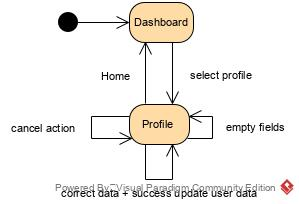
\includegraphics[width=\textwidth]{images/diagramma-macchine-stati/update-user-data}
\end{figure}

\begin{figure}[H]
	\centering
	\caption{Diagramma macchine a stati del caso d'uso 'View report of a 
	video'.}
	\label{fig:diagramma-macchine-stati:view-report-video}
	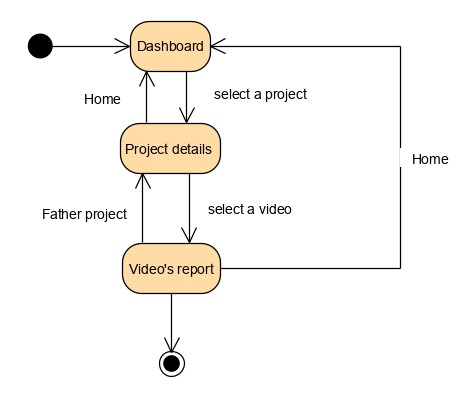
\includegraphics[width=\textwidth]{images/diagramma-macchine-stati/view-report-video}
\end{figure}

\begin{figure}[H]
	\centering
	\caption{Diagramma macchine a stati del caso d'uso 'View report of a 
	project'.}
	\label{fig:diagramma-macchine-stati:view-report-project}
	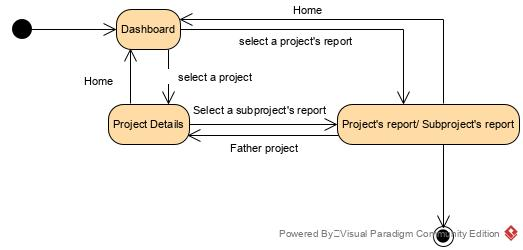
\includegraphics[width=\textwidth]{images/diagramma-macchine-stati/view-report-project}
\end{figure}

\begin{figure}[H]
	\centering
	\caption{Diagramma macchine a stati del caso d'uso 'Download report'.}
	\label{fig:diagramma-macchine-stati:download-report}
	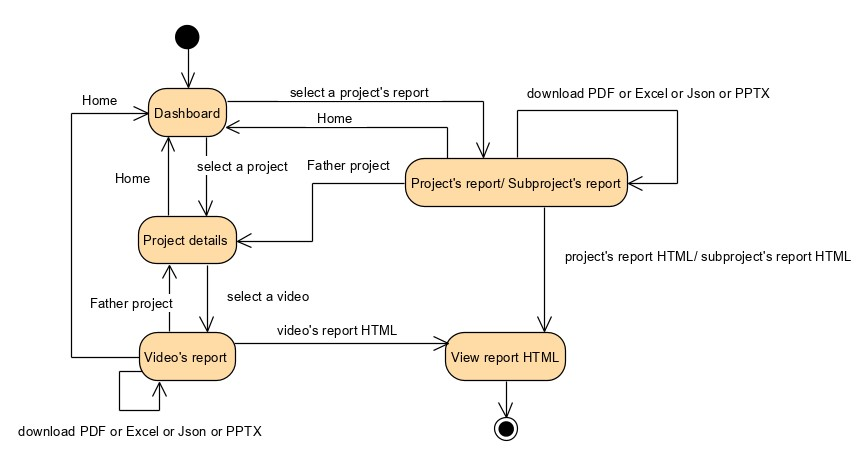
\includegraphics[width=\textwidth]{images/diagramma-macchine-stati/download-report}
\end{figure}